\scanpage{48}
une grosse variation modulaire de $X_0$, s'exprimant disons par le fait que $X_0$ est la fibre, en un point $t_0$ au dessus du pt fermé $s_0$ de $S$, d'un schéma propre et lisse \inserted{$Y$} sur un $M$ de type fini sur $S$.
\figure{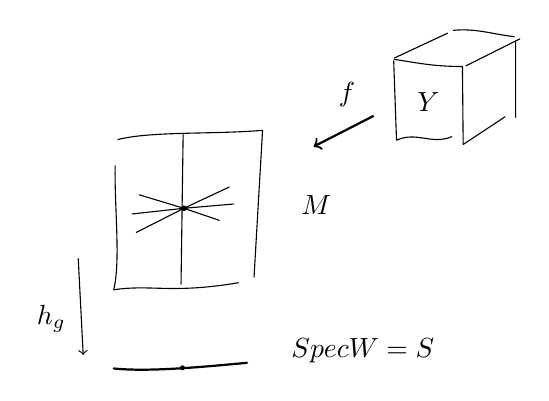
\begin{tikzpicture}[x=.009cm,y=-.009cm,line cap=round,line join=round]
\draw (554,335)--(629,300) (637,296) .. controls (669,293) and (691,301) .. (723,305);
\draw (554,337) .. controls (582,341) and (607,347) .. (650,347);
\draw (655,346)--(731,308) (725,312)--(725,419);
\draw (553,339)--(557,451) .. controls (585,438) and (606,458) .. (635,446);
\draw (650,348)--(651,457)--(710,418);
\node at (602,397) {$Y$};
\draw[->,thick] (524,417)--(440,460);
\node at (487,386) {$f$};
\draw (164,450) .. controls (211,438) and (300,443) .. (368,437)--(356,644);
\draw (160,487) .. controls (159,547) and (168,621) .. (158,662) .. controls (210,654) and (240,668) .. (334,652);
\draw (256,441)--(253,654) (194,528)--(257,547)--(307,564) (190,581)--(257,547)--(321,517) (184,555)--(257,547)--(327,541);
\fill (257,547) circle[radius=4];
\node at (444,542) {$M$};
\draw[->] (108,618)--(115,754);
\node at (70,703) {$h_{\deleted{\unsure{g}}}$};
\draw[thick] (158,773) .. controls (208,778) and (281,771) .. (346,765);
\fill (255,772) circle[radius=3.5];
\node[anchor=west] at (395,748) {$\operatorname{Spec} W=S$};
\end{tikzpicture}}
Les différentes sections de $M$ sur $S$ donneront différentes façons de relever $X_0$ en un $X$ propre et lisse sur $S$. Posant
\begingroup\makeatletter\tagsleft@true\makeatother
\[
K^{\bullet}=Rf_*(\underline{\Omega}^{\cdot}_{Y/M}) \tag*{(*)}
\]
\endgroup
on voit que pour tt telle section $g$ de $M$ sur $S$, définissant un $X^{\deleted{\unsure{(g)|g|(\Sigma)}}}_g$, et
\[
f^{\deleted{\unsure{(g)|g|(\Sigma)}}}_g : X^{\deleted{(\Sigma)}}_g \longrightarrow S
\]
% slanted
\margin{$\substack{\unsure{=}\\ (k\unsure{+|-}\frac{1}{2})\log(k+1)\\ =-(k-\frac{1}{2})\unsure{\mathrm{lo}|\log}}$}
on a
\[
\mathbb{R}f_{g*}(\underline{\Omega}^{*}_{X_g/S})
\xleftarrow[\substack{\text{isom}\\\text{can}}]{\sim} g^*(K^{\cdot})
\]
($g^*$ au sens des catégories dérivées .... ). Il s'ensuit, du moins modulo torsion, que
\[
\mathbb{R}^{i} f_{g*}(\underline{\Omega}^{*}_{X_g/S})
\xleftarrow{\sim}g^{*}(\mathscr{H}^{i})
\]
% archive sheet number: 47

